% ==========================================
% BAB V EVALUASI
% ==========================================
\cleardoublepage
\chapter{EVALUASI}
\label{chap:V}

Evaluasi merupakan tahap kelima DSRM \cite{Peffers2007} yang menilai artefak penelitian sebelum diimplementasikan. Artefak yang dievaluasi adalah TOGAF Pertahanan Indonesia pada Bab III serta arsitektur transformasi digital Kemhan RI beserta rencana migrasinya pada Bab IV. Evaluasi dilakukan melalui tiga pendekatan, yaitu evaluasi teoretis, evaluasi praktis, dan evaluasi komparatif, sebagaimana ditunjukkan pada Gambar~\ref{fig:V.1}.
\begin{figure}[htbp]
\centering
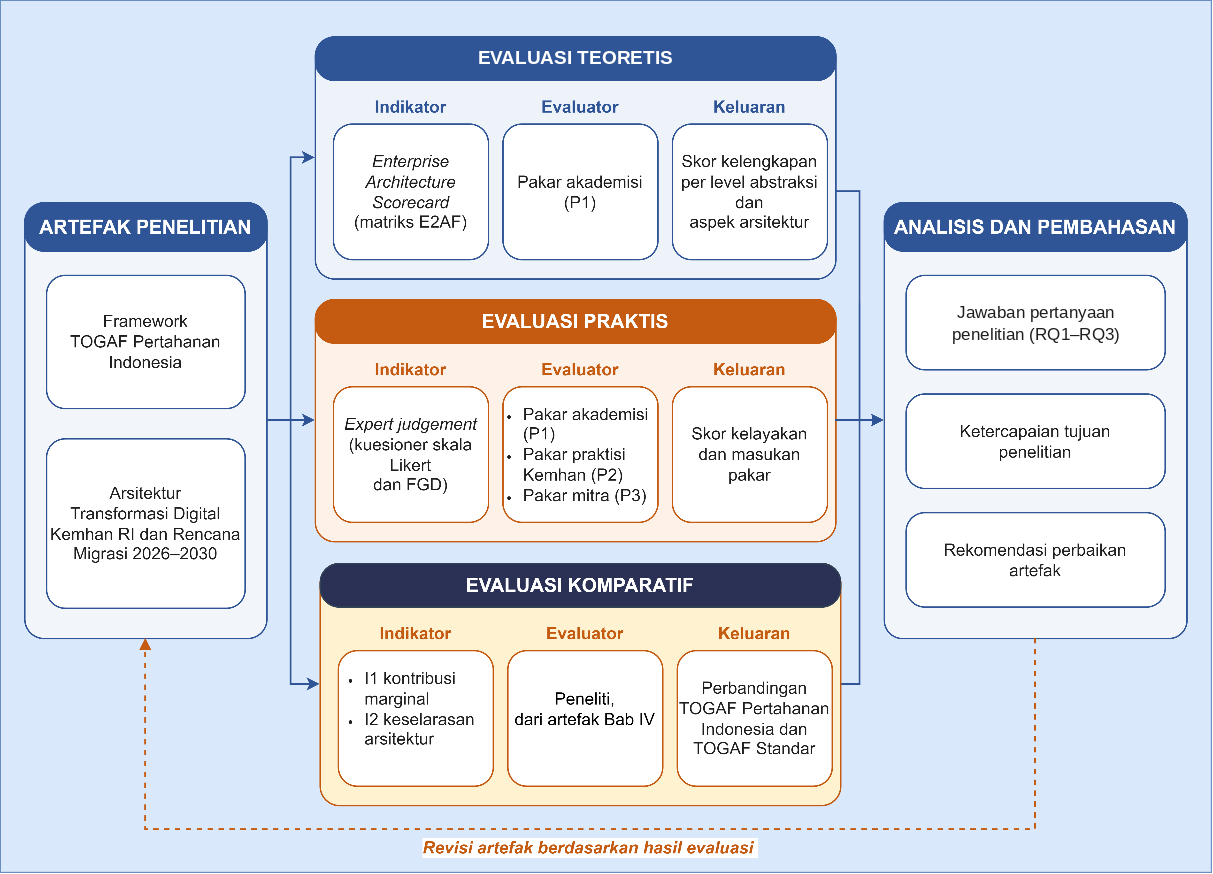
\includegraphics[width=0.99\linewidth,height=0.8\textheight,keepaspectratio]{images/Alur Evaluasi Artefak Penelitian.png}
\caption{Alur Evaluasi Artefak Penelitian}
\label{fig:V.1}
\end{figure}

Gambar~\ref{fig:V.1} menunjukkan bahwa ketiga pendekatan dijalankan terhadap artefak yang sama. Evaluasi teoretis dan evaluasi praktis dilakukan oleh pakar, sedangkan evaluasi komparatif dihitung peneliti dari artefak pada Bab IV. Hasil ketiganya dipadukan untuk menjawab pertanyaan penelitian dan dikembalikan ke artefak sebagai bahan perbaikan.

\section{Rancangan Evaluasi}
\label{sec:V.1}

Rancangan evaluasi meliputi objek dan pendekatan evaluasi, pemilihan pakar, serta instrumen dan teknik analisis.

\subsection{Objek dan Pendekatan Evaluasi}
\label{sec:V.1.1}

Objek evaluasi terdiri atas dua jenis artefak \textit{design science}, yaitu metode dan instansiasi \cite{Hevner2004}. Artefak metode adalah TOGAF Pertahanan Indonesia, sedangkan artefak instansiasi adalah arsitektur transformasi digital Kemhan RI. RQ1 dan RQ2 dijawab melalui perancangan pada Bab III dan penerapan pada Bab IV, sedangkan evaluasi pada bab ini menjawab RQ3, yaitu kelayakan framework dan arsitektur serta kontribusinya dibandingkan TOGAF ADM standar. Rancangan ketiga pendekatan evaluasi disajikan pada Tabel~\ref{tab:V.1}.

\begingroup\small\setstretch{1.0}
\begin{longtable}{@{}>{\raggedright\arraybackslash\hspace{0pt}}p{0.168\linewidth}>{\raggedright\arraybackslash\hspace{0pt}}p{0.246\linewidth}>{\raggedright\arraybackslash\hspace{0pt}}p{0.246\linewidth}>{\raggedright\arraybackslash\hspace{0pt}}p{0.246\linewidth}@{}}
\caption{Rancangan Evaluasi}\label{tab:V.1}\\
\toprule
\textbf{Unsur} & \textbf{Evaluasi Teoretis} & \textbf{Evaluasi Praktis} & \textbf{Evaluasi Komparatif}\\
\midrule
\endfirsthead
\multicolumn{4}{@{}l}{\small\itshape \tablename\ \thetable{} (lanjutan)}\\
\toprule
\textbf{Unsur} & \textbf{Evaluasi Teoretis} & \textbf{Evaluasi Praktis} & \textbf{Evaluasi Komparatif}\\
\midrule
\endhead
\bottomrule
\endlastfoot
Tujuan & Menilai kelengkapan dokumentasi arsitektur & Menilai kelayakan penerapan framework dan arsitektur di Kemhan RI & Mengukur kontribusi modifikasi dibandingkan TOGAF ADM standar\\
Instrumen & Enterprise Architecture Scorecard \cite{Schekkerman2004} & Kuesioner skala Likert 1–5 dan FGD & Indikator I1 dan I2\\
Evaluator & Pakar akademisi (P1) & Pakar akademisi (P1), pakar praktisi (P2), dan pakar mitra (P3) & Peneliti\\
Teknik analisis & Persentase skor per level abstraksi dan area aspek & Rata-rata skor, indeks Aiken’s V, dan analisis masukan pakar & Penelusuran asal kesenjangan dan pemetaan domain Arsitektur SPBE\\
Keluaran & Kategori kelengkapan dan butir yang perlu diperbaiki & Kategori kelayakan dan rekomendasi perbaikan & Kontribusi komponen hasil modifikasi dan keselarasan SPBE\\
Target (Subbab I.6) & Kategori Baik & Kategori Layak & –\\
Bagian RQ3 yang dijawab & Kelayakan arsitektur dari sisi dokumentasi & Kelayakan framework dan arsitektur dari sisi penerapan & Kontribusi dibandingkan TOGAF ADM standar\\
\end{longtable}
\endgroup

Tabel~\ref{tab:V.1} menunjukkan bahwa kelayakan dinilai dari sisi dokumentasi dan penerapan, sedangkan kontribusi dinilai melalui perbandingan dengan TOGAF ADM standar. Ketiga pendekatan bersifat \textit{ex-ante} sesuai Subbab~\ref{sec:I.5}, sehingga yang dinilai adalah kualitas rancangan. Dampak implementasi diukur kemudian oleh Kemhan RI melalui indikator pada Tabel~\ref{tab:IV.40}.

\subsection{Pemilihan Pakar}
\label{sec:V.1.2}

Pakar dipilih secara terencana\textit{,} yaitu berdasarkan kesesuaian keahlian dan pengalaman dengan objek evaluasi. Kriteria pemilihannya adalah memiliki latar belakang pendidikan atau jabatan di bidang \textit{enterprise architecture}, SPBE, teknologi informasi, atau sistem pertahanan; berpengalaman paling sedikit lima tahun pada bidang tersebut; serta memahami transformasi digital di lingkungan Kemhan RI, sektor pemerintahan, atau industri pertahanan. Pakar dikelompokkan ke dalam tiga kategori agar artefak dinilai dari sudut pandang akademik, internal organisasi, dan eksternal, sebagaimana disajikan pada Tabel~\ref{tab:V.2}.

\begingroup\small\setstretch{1.0}
\begin{longtable}{@{}>{\raggedright\arraybackslash\hspace{0pt}}p{0.076\linewidth}>{\raggedright\arraybackslash\hspace{0pt}}p{0.224\linewidth}>{\raggedright\arraybackslash\hspace{0pt}}p{0.193\linewidth}>{\raggedright\arraybackslash\hspace{0pt}}p{0.103\linewidth}>{\raggedright\arraybackslash\hspace{0pt}}p{0.136\linewidth}>{\raggedright\arraybackslash\hspace{0pt}}p{0.115\linewidth}@{}}
\caption{Profil Pakar per Kategori}\label{tab:V.2}\\
\toprule
\textbf{Kode} & \textbf{Kategori dan Unsur} & \textbf{Sudut Pandang Penilaian} & \textbf{Jumlah} & \textbf{Pengalaman} & \textbf{Instrumen}\\
\midrule
\endfirsthead
\multicolumn{6}{@{}l}{\small\itshape \tablename\ \thetable{} (lanjutan)}\\
\toprule
\textbf{Kode} & \textbf{Kategori dan Unsur} & \textbf{Sudut Pandang Penilaian} & \textbf{Jumlah} & \textbf{Pengalaman} & \textbf{Instrumen}\\
\midrule
\endhead
\bottomrule
\endlastfoot
\centering\arraybackslash P1 & Pakar Akademisi: dosen atau peneliti perguruan tinggi, seperti ITB dan Universitas Pertahanan RI & Ketepatan konseptual terhadap kaidah \textit{enterprise architecture} dan TOGAF & \centering\arraybackslash \ldots{} & \centering\arraybackslash \ldots{} & Kuesioner dan EA Scorecard\\
\centering\arraybackslash P2 & Pakar Praktisi: pejabat atau staf Kemhan RI, seperti Pusat Data dan Informasi, Ditjen Potensi Pertahanan, dan Badan Informasi dan Komunikasi Intelijen Pertahanan & Kesesuaian dengan kondisi dan kebutuhan organisasi & \centering\arraybackslash \ldots{} & \centering\arraybackslash \ldots{} & Kuesioner\\
\centering\arraybackslash P3 & Pakar Mitra: industri pertahanan, BUMN/BUMS, atau lembaga mitra Kemhan RI & Kelayakan dari sisi penyedia teknologi, termasuk biaya, risiko, dan interoperabilitas C6ISR & \centering\arraybackslash \ldots{} & \centering\arraybackslash \ldots{} & Kuesioner\\
 & \textbf{Jumlah} &  & \centering\arraybackslash \textbf{\ldots{}} &  & \\
\end{longtable}
\endgroup

Tabel~\ref{tab:V.2} menunjukkan bahwa seluruh pakar mengisi kuesioner \textit{expert judgement}, sedangkan Enterprise Architecture Scorecard hanya diisi pakar akademisi karena memerlukan pemahaman matriks E2AF. Identitas pakar disamarkan dan disajikan per kategori.

\subsection{Instrumen dan Teknik Analisis}
\label{sec:V.1.3}

Evaluasi dilaksanakan melalui FGD yang dipisahkan per kategori pakar. Setiap sesi menggunakan materi, urutan pemaparan, dan instrumen yang sama agar hasil antarsesi dapat dibandingkan. Materi utamanya adalah dokumen \textit{Kajian Arsitektur Transformasi Digital Kementerian Pertahanan Republik Indonesia Menuju Pertahanan Cerdas}, yaitu ringkasan Bab III dan Bab IV yang dilengkapi latar belakang permasalahan. Setiap butir instrumen dilengkapi rujukan bagian dan halaman Kajian, sedangkan pakar akademisi juga memperoleh naskah lengkap.

Setiap sesi terdiri atas empat langkah, yaitu pemaparan artefak, pengisian instrumen pada akhir sesi, pencatatan komentar dan hasil diskusi, serta analisis hasil untuk menentukan bagian artefak yang dipertahankan atau disempurnakan. Instrumen diisi melalui formulir daring yang terhubung dengan lembar kerja analisis, sedangkan formulir cetak disediakan sebagai cadangan.

\subsubsection{\textit{Enterprise Architecture Scorecard}}
\label{sec:V.1.3.1}

\textit{Enterprise Architecture Scorecard} dikembangkan oleh \textit{Schekkerman} untuk menilai kualitas dokumentasi arsitektur \textit{enterprise} \cite{Schekkerman2004,Schekkerman2006}. Instrumen ini menggunakan matriks \textit{Extended Enterprise Architecture Framework} (E2AF) yang terdiri atas empat area aspek, yaitu bisnis, informasi, sistem informasi, dan infrastruktur teknologi, serta enam level abstraksi, yaitu \textit{contextual}, \textit{environmental}, \textit{conceptual}, \textit{logical}, \textit{physical}, dan \textit{transformational}. Instrumen terdiri atas 35 butir. Setiap butir dinilai dengan tiga status, yaitu 0 apabila belum terdokumentasi, 1 apabila terdokumentasi sebagian, dan 2 apabila terdokumentasi dengan baik.

Karena TOGAF Pertahanan Indonesia menambahkan domain C6ISR, instrumen disesuaikan menjadi lima area aspek, yaitu bisnis, data, aplikasi, teknologi, dan C6ISR, ditambah satu kolom keselarasan antararea. Dengan demikian, setiap butir dinilai pada enam kolom. Skor dihitung dengan persamaan berikut.

\begin{equation}
\text{Skor maksimum} = n \times 6 \times 2
\eqcaption{Skor maksimum}
\label{eq:V.1}
\end{equation}

\begin{equation}
\text{Persentase skor} = (\Sigma\ \text{skor diperoleh} \div \text{skor maksimum}) \times 100\%
\eqcaption{Persentase skor}
\label{eq:V.2}
\end{equation}

dengan \textit{n} adalah jumlah butir pada level abstraksi yang dinilai. Skor diperoleh merupakan rata-rata status dari seluruh pakar akademisi. Karena instrumen asli tidak menetapkan batas kategori, batas kategori ditetapkan peneliti sebagaimana disajikan pada Tabel~\ref{tab:V.3}, sedangkan butir berstatus 1 ditelaah lebih lanjut sebagai bahan perbaikan.

\begingroup\small\setstretch{1.0}
\begin{longtable}{@{}>{\raggedright\arraybackslash\hspace{0pt}}p{0.214\linewidth}>{\raggedright\arraybackslash\hspace{0pt}}p{0.167\linewidth}>{\raggedright\arraybackslash\hspace{0pt}}p{0.555\linewidth}@{}}
\caption{Kategori Interpretasi Skor \textit{Enterprise Architecture Scorecard}}\label{tab:V.3}\\
\toprule
\textbf{Persentase Skor} & \textbf{Kategori} & \textbf{Makna}\\
\midrule
\endfirsthead
\multicolumn{3}{@{}l}{\small\itshape \tablename\ \thetable{} (lanjutan)}\\
\toprule
\textbf{Persentase Skor} & \textbf{Kategori} & \textbf{Makna}\\
\midrule
\endhead
\bottomrule
\endlastfoot
\centering\arraybackslash $\geq$ 80\% & \centering\arraybackslash Baik & Arsitektur terdokumentasi lengkap dan dapat dijadikan acuan\\
\centering\arraybackslash 60\% – < 80\% & \centering\arraybackslash Cukup & Arsitektur dapat digunakan dengan perbaikan pada butir tertentu\\
\centering\arraybackslash < 60\% & \centering\arraybackslash Kurang & Arsitektur memerlukan perbaikan mendasar sebelum digunakan\\
\end{longtable}
\endgroup

Tabel~\ref{tab:V.3} menunjukkan bahwa target kategori Baik pada Subbab~\ref{sec:I.6} setara dengan persentase skor minimal 80\%.

\subsubsection{Kuesioner \textit{Expert Judgement}}
\label{sec:V.1.3.2}

Kuesioner \textit{expert judgement} menilai kelayakan framework dan arsitektur untuk diterapkan di lingkungan Kemhan RI. Kuesioner terdiri atas 24 pernyataan dalam tujuh aspek, yaitu:
\begin{enumerate}[label=\arabic*.]
\item Kelayakan framework TOGAF Pertahanan Indonesia (aspek A);
\item Relevansi Fase C6ISR Architecture (aspek B);
\item Efisiensi proses (aspek C);
\item Interoperabilitas sistem (aspek D);
\item Keamanan dan kesiapan pengelolaan data (aspek E);
\item Kelayakan adopsi dalam organisasi (aspek F); dan
\item Kelayakan \textit{roadmap} dan rencana migrasi (aspek G).
\end{enumerate}

Pernyataan B3 dan B4 meminta pakar membandingkan arsitektur yang dihasilkan dengan penerapan TOGAF ADM standar, sehingga menjadi bukti pakar bagi evaluasi komparatif. Setiap pernyataan dinilai dengan skala Likert 1–5, dari sangat tidak setuju hingga sangat setuju, dan dilengkapi kolom komentar. Seluruh pernyataan disajikan pada Lampiran A.2.

Analisis dilakukan dalam dua tahap. Rata-rata skor digunakan untuk menentukan tingkat kelayakan, sedangkan indeks Aiken’s V digunakan untuk menilai validitas isi setiap pernyataan \cite{Aiken1985}. Indeks Aiken’s V dihitung dengan persamaan berikut.

\begin{equation}
V = \Sigma s \div [n(c - 1)], \quad \text{dengan } s = r - \mathit{lo}
\eqcaption{Indeks Aiken’s V}
\label{eq:V.3}
\end{equation}

dengan \textit{r} adalah skor dari pakar, \textit{lo} adalah skor terendah (1), \textit{n} adalah jumlah pakar, dan \textit{c} adalah jumlah kategori penilaian (5). Pernyataan dinyatakan valid apabila nilai \textit{V} memenuhi nilai kritis sesuai jumlah pakar dan jumlah kategori. Pada taraf signifikansi 5\%, nilai kritis \textit{V} adalah 0,75 untuk tujuh atau delapan pakar dan 0,72 untuk sembilan pakar \cite{Aiken1985}.

Rata-rata dan Aiken’s V dihitung dari seluruh pakar secara perorangan sehingga setiap pakar memiliki bobot yang sama. Rata-rata setiap aspek juga dihitung per kategori pakar sebagai pelengkap. Rata-rata skor kemudian diterjemahkan ke dalam kategori kelayakan pada Tabel~\ref{tab:V.4}.

\begingroup\small\setstretch{1.0}
\begin{longtable}{@{}>{\raggedright\arraybackslash\hspace{0pt}}p{0.483\linewidth}>{\raggedright\arraybackslash\hspace{0pt}}p{0.483\linewidth}@{}}
\caption{Kategori Interpretasi Skor Kelayakan}\label{tab:V.4}\\
\toprule
\textbf{Rentang Rata-rata} & \textbf{Kategori}\\
\midrule
\endfirsthead
\multicolumn{2}{@{}l}{\small\itshape \tablename\ \thetable{} (lanjutan)}\\
\toprule
\textbf{Rentang Rata-rata} & \textbf{Kategori}\\
\midrule
\endhead
\bottomrule
\endlastfoot
\centering\arraybackslash 1,00 – 1,80 & \centering\arraybackslash Sangat tidak layak\\
\centering\arraybackslash 1,81 – 2,60 & \centering\arraybackslash Tidak layak\\
\centering\arraybackslash 2,61 – 3,40 & \centering\arraybackslash Cukup layak\\
\centering\arraybackslash 3,41 – 4,20 & \centering\arraybackslash Layak\\
\centering\arraybackslash 4,21 – 5,00 & \centering\arraybackslash Sangat layak\\
\end{longtable}
\endgroup

\subsubsection{Indikator Evaluasi Komparatif}
\label{sec:V.1.3.3}

Evaluasi komparatif membandingkan dua versi arsitektur Kemhan RI. Versi A adalah arsitektur yang disusun dengan TOGAF Pertahanan Indonesia pada Bab IV. Versi B mewakili penerapan TOGAF ADM standar pada kasus yang sama, yaitu Versi A tanpa komponen bertanda Δ dan + pada Tabel~\ref{tab:III.7} hingga Tabel~\ref{tab:III.15}. Kedua indikator berikut dihitung peneliti dari artefak yang tersedia, sehingga tidak menambah butir kuesioner.
\begin{enumerate}[label=\arabic*.]
\item I1 – Kontribusi marginal, yaitu jumlah kesenjangan yang dikonsolidasikan pada Tabel~\ref{tab:IV.33} dan paket pekerjaan pada Tabel~\ref{tab:IV.34} yang hanya teridentifikasi karena komponen bertanda Δ atau +. Indikator ini menunjukkan hal yang akan terlewat apabila arsitektur disusun dengan TOGAF ADM standar.
\item I2 – Keselarasan SPBE, yaitu proporsi domain Arsitektur SPBE yang tercakup dalam setiap versi. Domain tersebut meliputi proses bisnis, data dan informasi, aplikasi, infrastruktur, keamanan, dan layanan \cite{Perpres132Tahun2022}. Indikator ini memastikan bahwa penambahan muatan pertahanan tidak mengurangi keselarasan dengan SPBE.
\end{enumerate}

\begin{equation}
\text{I2} = (\text{jumlah domain SPBE yang tercakup} \div 6) \times 100\%
\eqcaption{Keselarasan SPBE (I2)}
\label{eq:V.4}
\end{equation}

Sebagai pelengkap, rata-rata pernyataan B3 dan B4 digunakan sebagai bukti pakar atas kontribusi komponen hasil modifikasi.

\section{Evaluasi Teoretis dengan Enterprise Architecture Scorecard}
\label{sec:V.2}

\subsection{Pemetaan Artefak ke Matriks E2AF}
\label{sec:V.2.1}

\subsection{Hasil Penilaian}
\label{sec:V.2.2}

\section{Evaluasi Praktis melalui \textit{Expert Judgement}}
\label{sec:V.3}

\subsection{Pelaksanaan Evaluasi}
\label{sec:V.3.1}

\subsection{Hasil Penilaian Kelayakan}
\label{sec:V.3.2}

\subsection{Masukan Pakar dan Tindak Lanjut}
\label{sec:V.3.3}

\section{Evaluasi Komparatif terhadap TOGAF ADM Standar}
\label{sec:V.4}

\section{Pembahasan}
\label{sec:V.5}

\subsection{Ketercapaian Tujuan dan Keluaran Penelitian}
\label{sec:V.5.1}

\subsection{Kontribusi Modifikasi TOGAF Berbasis C6ISR}
\label{sec:V.5.2}

\subsection{Keterbatasan Penelitian}
\label{sec:V.5.3}
